\chapter{Interaktion per GUI}
\chplbl{bed-gui}
Der zweite Teil der Aufgabe war es, eine grafische Oberfläche für den \md{} zu entwickeln -- die \mdg{}. Wie diese bedient wird, worauf Du achten solltest und wie sich die \mdg{} vom \md{} unterscheidet werde ich in diesem Kapitel erläutern. Am Ende des Kapitels biete ich wie für den \md{} ein Tutorial an, welches Dir die Funktionsweise der \mdg{} an einem Beispiel nahebringen soll.

Auch die \mdg{} erfordert keine Installation und besteht nur aus einer \datei{zip}, die Du entpacken musst. Die Schritte vom Herunterladen bis zum Starten der \mdg{} sind dabei analog zum \md{}:

\begin{enumerate}
\item Die Datei \texttt{micro-debug-gui-version.zip} von der Projektseite\notiz{Verweis auf Seite} herunterladen
\item Die \datei{zip} in ein beliebiges Verzeichnis entpacken (bspw. \texttt{/opt/micro-debug-gui/})
\item Das Verzeichnis der \mdg{} dem \texttt{PATH} hinzufügen
\item Die \mdg{} starten -- mit \texttt{\$ micro-debug-gui.sh -{}-help}
\end{enumerate}

Die grafische Oberfläche ist technisch eine eigenständige Anwendung, die die Konsolenvariante benutzt -- wie ich in \chpref{gui} erläutere. Demzufolge enthält die grafische Oberfläche auch den Code der Konsolenvariante des \md{} -- dadurch kannst Du mit ein wenig Anpassung auch die Konsolenvariante nutzen. Dies möchte ich nun kurz etwas vertiefen.

\section{Nutzung der Konsolenvariante}
\seclbl{gui-nutzung-konsole}
Nach dem Entpacken der \datei{zip} entsteht eine ähnliche Verzeichnis-Struktur, wie beim \md{}. Allerdings existiert nun das Verzeichnis \texttt{lib/}, das unter anderem eine \datei{jar} beinhaltet, die den Code des \md{} enthält -- die Datei \texttt{micro-debug-version.jar}.

Ich möchte nun zeigen, wie man die \mdg{} so ergänzt, dass sowohl die \mdg{} als auch der \md{} aufrufbar sind. Da dieses Verhalten für Windows und Linux analog ist, zeige ich es am Beispiel von Linux, wie in \lstref{parallele-nutzung-md-mdg} vorbereitet.

\begin{lstlisting}[language=sh,caption={Parallele Nutzung des \md{} und der \mdg{}},label=\lstlbl{parallele-nutzung-md-mdg}]
cd micro-debug-gui-version/
cp micro-debug-gui.sh micro-debug.sh
\end{lstlisting}

Als Basis für die parallele Nutzung kopiere das Startskript der \mdg{}; diese Kopie (\texttt{micro-debug.sh}) musst Du nun noch anpassen:
\begin{enumerate}
\item Ersetze \texttt{"\$DIR/micro-debug-gui-versiong.jar":"\$DIR/lib/*"} durch \texttt{"\$DIR/lib/micro-debug-versionk.jar"}, wobei \emph{versiong} die Version der \mdg{} und \emph{versionk} die Version des \md{} ist.
\item Ersetze \texttt{com.github.croesch.micro_debug.gui.MicroDebug} durch \texttt{com.github.croesch.micro_debug.MicroDebug}
\end{enumerate}

Nach diesen Schritten hast Du zwei Startskripte: Eines zum Start der \mdg{} und eines zum Start des \md{}. Beide kannst Du nun unabhängig voneinander ausführen.

\section{Unterschiede zur Konsolenvariante}
Wie Du bemerkt hast, ist die Struktur von \md{} und \mdg{} ähnlich, aber nicht gleich. Auch beim Aufruf und bei der Bedienung gibt es einige nennenswerte Unterschiede, die ich Dir nun zeigen möchte.

\subsection{Parameter}
\seclbl{unterschied-parameter}
Schon der Aufruf der \mdg{} unterscheidet sich von dem des \md{}: Es gibt weniger Parameter und Du kannst die \mdg{} auch ohne Parameter aufrufen, alle der folgenden Parameter sind also optional.

\begin{description}
\item[-h, -{}-help]
  mit diesem Parameter kannst Du dir wie beim \md{} die Hilfe anzeigen lassen, die neben den verschiedenen Aufrufmöglichkeiten die möglichen Parameter erklärt. Zusätzlich werden auch hier noch einige andere Informationen, wie Kontaktmöglichkeiten, angezeigt.

\item[-v, -{}-version]
  gibt die Version der \mdg{} und des benutzten \md{} aus.
\end{description}

Wie beim \md{} startet der Debugger nicht, wenn Du dir die Hilfe oder Versionsnummern anzeigen lässt, sondern beendet sich nach Ausgabe der Informationen.

Anders als der \md{} benötigt die \mdg{} die Pfade zu den Bytecode-Dateien nicht; diese werden direkt zu Beginn über die grafische Oberfläche eingegeben. Dies erkläre ich nochmal genauer im \secref{startfenster}.

\subsection{Verfügbare Funktionen}
Die \mdg{} benutzt den \md{} und hat daher prinzipiell Zugriff auf alle Funktionen, die der \md{} dem Benutzer bereitstellt. Da die \mdg{} dem Benutzer aber fortlaufend die Werte der Register und des Hauptspeichers, den Mikro-Assembler- sowie den Assembler-Code anzeigt, ist es nicht nötig diese Werte beobachten zu können. Befehle wie \texttt{trace-reg} wirst Du daher in der \mdg{} nicht wiederfinden. Auch die Ausgabe des Stacks gibt es nicht mehr, denn dieser kann im Hauptspeicher angesehen werden.

Auch die Breakpoints werden dem Benutzer fortlaufend angezeigt und können über Mausklicks aktiviert/deaktiviert werden, daher fallen Befehle wie \texttt{ls-break} auch weg.

Wie wir gerade gesehen haben, bietet die \mdg{} konstruktionsbedingt manche Funktionen nicht explizit an. Es gibt aber auch manche Funktionen, die bisher noch gar nicht über die \mdg{} abgebildet sind, diese sind:
\begin{itemize}
\item Einen Breakpoint für einen bestimmten Wert eines Registers zu setzen (\texttt{break Register Wert}).
\item eine gewisse Anzahl an (Mikro-)Instruktionen auszuführen, per \texttt{micro-step Zahl}.
\item den Wert eines Registers zu verändern, per \texttt{set Register Zahl}.
\item den Wert eines Wortes im Hauptspeicher zu setzen, per \texttt{set-mem Zahl1 Zahl2}.
\end{itemize}

Diese Funktionen habe ich bisher aus Zeitgründen noch nicht implementiert, werde ich aber nach und nach ergänzen.

\subsection{Geschwindigkeit}
Die \mdg{} nutzt die Funktionen des \md{}, um die \mic{} simulieren und debuggen zu können. Daraus folgt, dass die \mdg{} prinzipiell nicht schneller sein kann als der \md{}, sondern eher langsamer.

Diese Vermutung bestätigt sich, wenn man die \mdg{} benutzt. Bei einfachen Befehlen, wie eine (Mikro-)Instruktion auszuführen oder den Debugger zu resetten ist kein Geschwindigkeitsunterschied spürbar. Aber besonders bei dem \texttt{run}-Befehl ist deutlich zu beobachten, dass die \mdg{} langsamer ist.

Was macht die \mdg{} besonders langsam? Wahrscheinlich\footnote{Die Ursache für den Geschwindigkeitsverlust ist meine persönliche Vermutung. Wüsste ich es genau, dann wäre das Problem womöglich schon behoben.} ist die Ursache der langsamen Ausführung die Aktualisierung der Oberfläche: Die Werte der Register und des sichtbaren Hauptspeichers, sowie die aktuell ausgeführte Zeile werden ständig aktualisiert.

Ständig bedeutet, dass nach jedem Zyklus des Prozessors eine Aktualisierung durchgeführt wird. Ein wohl viel besseres Verhalten wäre, erst am Ende einer Ausführung die Aktualisierung durchzuführen. Besonders die Aktualisierung der aktuell ausgeführten Zeile wird die Aktualisierung der Oberfläche stark verlangsamen: Die Zeilennummernanzeige erhält die Hintergrundfarbe für die Hervorhebung über HTML-Code. Dieser Code wird bei jeder Änderung der aktuell hervorgehobenen Zeile neu erzeugt, was besonders bei vielen Zeilen deutlich unperformant wird.

Die \mdg{} bietet also nicht nur bei den angebotenen Funktionen Verbesserungsbedarf, sondern auch an der Geschwindigkeit. Im derzeitigen Zustand der \mdg{} lässt sich also gut sehen, welche Befehle nacheinander ausgeführt werden, aber die \mdg{} zum reinen Ausführen von Assembler-Code zu nutzen ist wohl zu unperformant.

\section{Oberflächenelemente}
Nachdem ich nun einige Eigenschaften der \mdg{} beschrieben habe, möchte ich Dir jetzt einen detaillierteren Einblick in die \mdg{} geben. Dazu werde ich die verschiedenen Hauptkomponenten der \mdg{} zeigen und deren Funktionen erklären.

\subsection{Startfenster}
\seclbl{startfenster}
Da wir, wie in \secref{unterschied-parameter} beschrieben, bei der \mdg{} die Pfade der Bytecode-Dateien nicht als Argumente übergeben, gibt es ein extra Fenster dafür. Dieses erscheint direkt nach dem Start der \mdg{} und ist in \figref{start-frame-empty} zu sehen.

\begin{figure}[h]
	\centering
	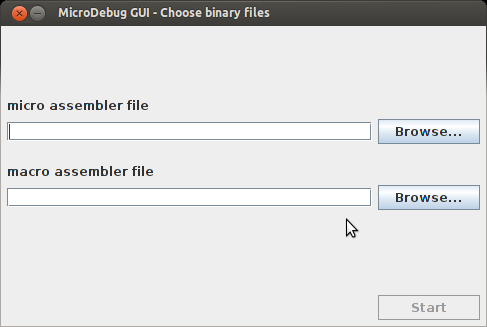
\includegraphics[width=6cm]{images/start-frame-empty}
	\caption{Screenshot des Start-Fensters}
	\figlbl{start-frame-empty}
\end{figure}

Hast Du zwei Pfade eingegeben, wird der Debugger über den Start-Button gestartet. In diesem Moment werden die beiden Bytecode-Dateien auf ihre Gültigkeit geprüft; zuerst die Mikro-Assembler-Datei und dann die Assembler-Datei. Falls eine der Dateien ungültig ist, wird statt dem Debugger erneut das Start-Fenster gezeigt. In diesem Fall ist dann das Textfeld mit der falschen Datei leer, wie beispielsweise in \figref{start-frame-both-wrong} zu sehen.

\begin{figure}[h]
	\centering
	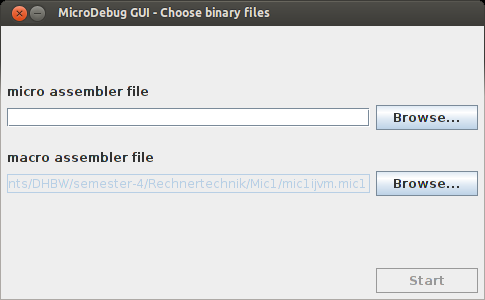
\includegraphics[width=6cm]{images/start-frame-both-wrong}
	\caption{Screenshot des Start-Fensters -- die angegebenen Dateien waren \emph{beide} ungültig}
	\figlbl{start-frame-both-wrong}
\end{figure}

In diesem Beispiel waren beide Dateien falsch, aber nur ein Textfeld ist leer. Die \mdg{} prüft die Dateien nacheinander, ist bereits die erste Datei ungültig, wird die zweite nicht geprüft und zunächst als gültig angenommen. Das Textfeld der zweiten Datei ist nun ausgegraut, Du kannst es aber mit einem Doppelklick wieder editierbar machen. In dem genannten Beispiel habe ich das getan und nun zwei korrekte Dateien eingetragen, wie Du in \figref{start-frame-both-filled} sehen kannst.

\begin{figure}[h]
	\centering
	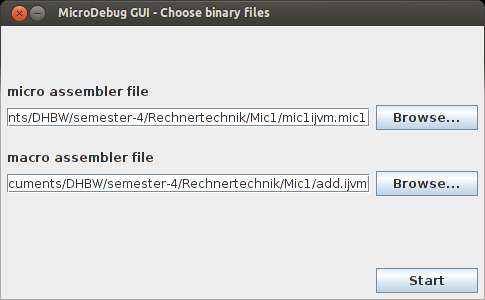
\includegraphics[width=6cm]{images/start-frame-both-filled}
	\caption{Screenshot des Start-Fensters mit zwei eingetragenen Dateien}
	\figlbl{start-frame-both-filled}
\end{figure}

Hast Du dann zwei korrekte Dateien eingetragen, startet der Debugger und du siehst das Hauptfenster aus \figref{main-frame-onbegin}.

\begin{figure}[h]
	\centering
	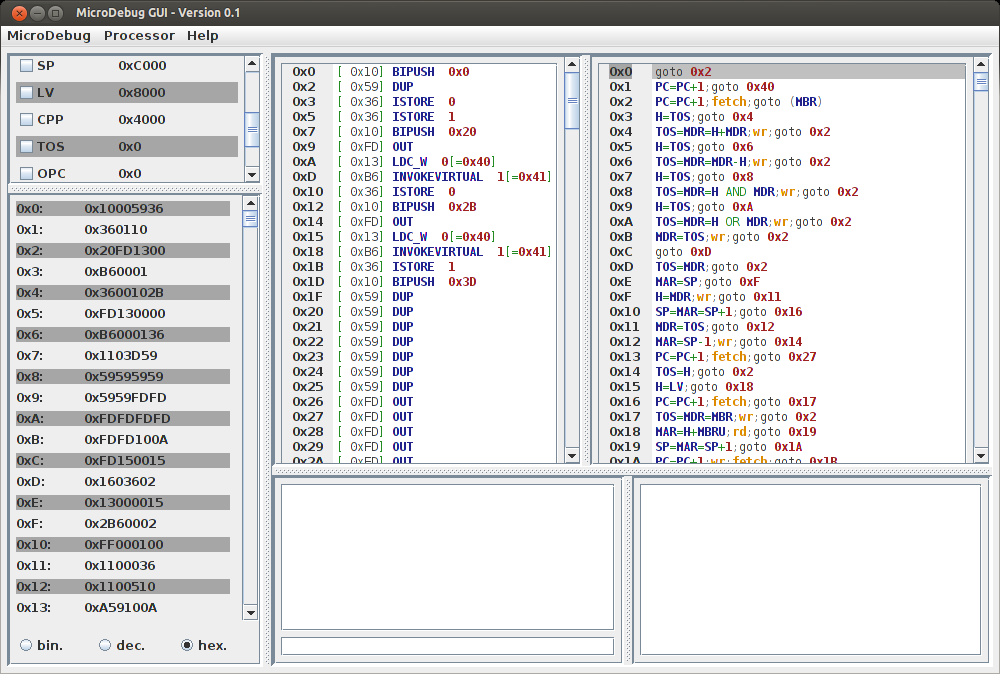
\includegraphics[width=0.8\linewidth]{images/main-frame-onbegin}
	\caption{Hauptfenster der \mdg{} zu Beginn}
	\figlbl{main-frame-onbegin}
\end{figure}

\subsection{Register}
In \figref{main-frame-onbegin} siehst Du links oben die Register mit ihren Werten, die gleiche Ansicht ist in \figref{main-frame-registers} nochmal größer dargestellt.

\begin{figure}[h]
	\centering
	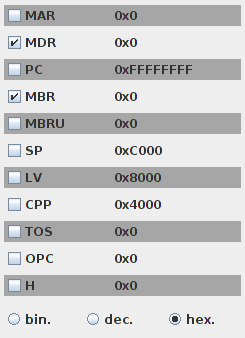
\includegraphics[width=4cm]{images/main-frame-registers}
	\caption{Registeransicht im Hauptfenster der \mdg{}}
	\figlbl{main-frame-registers}
\end{figure}

Die Checkboxen visualisieren die Breakpoints für die Register, in \figref{main-frame-registers} hält der Debugger demnach an, wenn \reg{MBR} oder \reg{MDR} im nächsten Zyklus geschrieben wird. Über die Radiobuttons unten kannst Du die Darstellung der Werte ändern, auf binär, dezimal oder hexadezimal -- so kannst Du für jeden Zweck die optimale Darstellung wählen.

\subsection{Hauptspeicher}
Unter der Registeransicht befindet sich im Hauptfenster die Ansicht des Hauptspeichers. Hier kannst du wie bei der Registeransicht die Darstellung der Hauptspeicherwerte jederzeit ändern.

In der Ansicht des Hauptspeichers sind nur eine feste Anzahl an Einträgen zu sehen, die sich nicht dynamisch an die Größe des sichtbaren Bereichs anpassen. Dies habe ich wegen der besseren Performanz so gelöst.

Die Ansicht zeigt den gesamten Hauptspeicher -- neben den lokalen Variablen, dem Stack und den Konstanten kannst Du auch den disassemblierten Assembler-Code in Bit-Form betrachten.

\subsection{Text-Ein- und -Ausgabe}
Rechts neben der Hauptspeicheransicht sind unten verschiedene Textareas zu sehen. Deren Funktion sollte dir spätestens im laufenden Betrieb des Debuggers deutlich werden: Links unten ist das Textfeld, um der \mic{} Text bereitzustellen, darüber befindet sich die Ausgabe der \mic{} und im rechten Bereich tauchen Informationen des \md{} auf, die auf der Konsole sichtbar waren und bisher noch keinen Platz in der Oberfläche bekommen haben.

\begin{figure}[h]
	\centering
	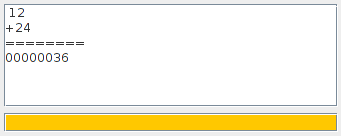
\includegraphics[width=4cm]{images/main-frame-mic-ta}
	\caption{Hauptspeicheransicht im Hauptfenster der \mdg{}}
	\figlbl{main-frame-mic-ta}
\end{figure}

\figref{main-frame-mic-ta} zeigt, wie sich das Eingabefeld verhält, wenn die \mic{} per \texttt{IN} ein Zeichen liest, aber der Puffer des \md{} keine Zeichen mehr enthält: es färbt sich orange. In diesem Fall solltest Du die nächste Eingabe eingeben und mit \emph{ENTER} bestätigen. Dadurch werden die eingegebenen Zeichen inklusive Zeilenumbruch im \md{} gepuffert, bis die \mic{} sie einliest.

Du kannst auch Eingaben machen, wenn der Puffer noch nicht leer ist, in diesem Fall wird der Text den du eingibst einfach dem Puffer des \md{} angehängt. So kannst Du schon beim Start des Programms bequem alle nötigen Eingaben machen und die \mdg{} die Eingaben abarbeiten lassen.

\subsection{Code}
Die wichtigsten zwei Komponenten befinden sich in \figref{main-frame-onbegin} rechts oben: Der disassemblierte Assembler- und Mikro-Assembler-Code. Die beiden Ansichten sind von der Funktion identisch aufgebaut und zeigen den disassemblierten Code mit Syntaxhervorhebung, Zeilennummern und den dazugehörigen Breakpoints an. Zusätzlich wird die Zeile des Codes hervorgehoben, die als nächstes ausgeführt wird.

\begin{figure}[h]
	\centering
	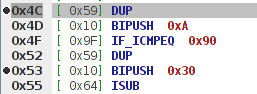
\includegraphics[width=4cm]{images/main-frame-code-part}
	\caption{Ausschnitt der Assembler-Code-Ansicht im Hauptfenster der \mdg{}}
	\figlbl{main-frame-code-part}
\end{figure}

\figref{main-frame-code-part} zeigt einen Ausschnitt der Code-Ansicht. Hier kannst Du sehen, dass als nächstes die Zeile \texttt{0x4C} abgearbeitet wird und dass in den Zeilen \texttt{0x4C} und \texttt{0x53} Breakpoints gesetzt sind. Die Breakpoints setzt und entfernst Du durch einen Doppelklick an die Stelle, an der sie gezeichnet werden -- links neben den Zeilennummern.


\section{Tutorial}